\documentclass[11]{article}
\usepackage{preamble}

\begin{document}
\pagenumbering{gobble}
\begin{titlepage}
	\begin{center}
		\vspace*{1cm}

		\Huge
		\textbf{AMME1362 Materials 1 - Assignment 5}

		\vspace{0.5cm}
		\LARGE
		\textbf{Due 05th October} \\
		Student Name: Josiah Tan\\
		Student Id:  500459959\\
		Tutor Name: DR. Naveed Aziz Khan\\
		Tutorial Class: 08

		\vspace{1.5cm}

		\large
		\vspace{1cm}

		\vfill

		\vspace{0.4cm}

		
\includegraphics[width=0.4\textwidth]{photos/university-of-sydney.png}

		\Large
		School of Aerospace, Mechanical and Mechatronic Engineering\\
		The University of Sydney\\
		Australia\\

		\newpage
		\tableofcontents % Not sure why the contents isn't centered 
	\end{center}
\end{titlepage}

\newpage
\large
\pagenumbering{arabic}
\section{Question 1}

% to get variables
% $1 + 2 = \getVariable{HelloWorld_c}$
% \getVariable{TestWriting_b}
% \getVariable{HelloWorld_c}

% to do the list
% There are many structural features that can influence mechanical properties of polymers.
% \begin{itemize}
% 	\item Side Groups
% 		Can be single atoms (H, O, F, Cl), branched carbon chains or an aromatic benzene ring.
% 	\item Polymer Chain Shape 
% 		Double bonding can restrict the ability of the polymer to rotate, thus affecting the mechanical properties
% \end{itemize}

% for two images
% \begin{figure}[H]%
%     \centering
%     \subfloat[\centering Horizontal]{{\includegraphics[width=0.475\textwidth]{photos/free_body_horizontal.png} }}%
%     \qquad
%     \subfloat[\centering Vertical]{{\includegraphics[width=0.475\textwidth]{photos/free_body_vertical.png} }}%
%     \caption{Free body, shear force and bending moment diagrams for two planes, the vertical is aligned in the direction of gravity, and the horizontal is aligned in the direction perpendicular to gravity}%
%     \label{fig:free_body}%
% \end{figure}

% for a single image
% \begin{figure}[h!]
% 	\centering
% 	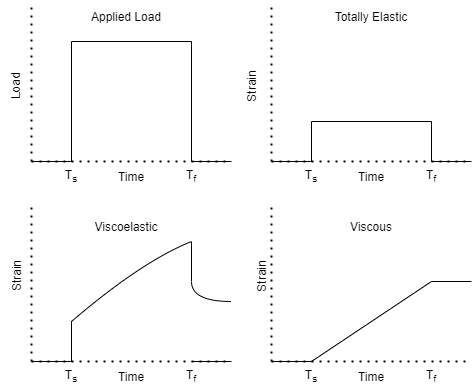
\includegraphics[width=0.75\textwidth]{photos/materials.png}
% 	\caption{Diagrams for totally elastic (top right), viscous (bottom right) and viscoelastic (bottom left)}
% 	\label{fig:al_li}
% \end{figure}

\cite{newton}

\bibliographystyle{IEEEtran}
\bibliography{main}
% \bibliography{main}
% \bibliographystyle{apalike}
\newpage
\end{document}



